
Este anexo proporciona una guía visual paso a paso para la utilización de la plataforma \textbf{Sky Apartments}. Se divide en dos secciones principales según el rol del usuario: la guía para huéspedes (navegación pública y gestión personal) y la guía para administradores (gestión del negocio).

\section{Guía para Huéspedes (Portal Público)}

\subsection{Página Principal (Home)}
La página de inicio de Sky Apartments ofrece la primera toma de contacto con la plataforma. Presenta los alojamientos más destacados, información sobre la empresa y un formulario de contacto directo para resolver dudas generales.

\begin{figure}[H]
    \centering
    \includegraphics[width=0.65\textwidth]{img/home.png}
    \caption{Página principal mostrando alojamientos destacados y formulario de contacto.}
\end{figure}

\subsection{Registro e Inicio de Sesión}
Para acceder a todas las funcionalidades del sistema (realizar reservas o dejar reseñas), es necesario disponer de una cuenta. 
\begin{itemize}
    \item Haga clic en el botón \textbf{"Sign Up"} en la esquina superior derecha para crear una cuenta nueva completando sus datos personales básicos y contraseña.
    \item Si ya dispone de cuenta, haga clic en \textbf{"Log In"} para acceder de forma segura a su panel.
\end{itemize}

\begin{figure}[H]
    \centering
    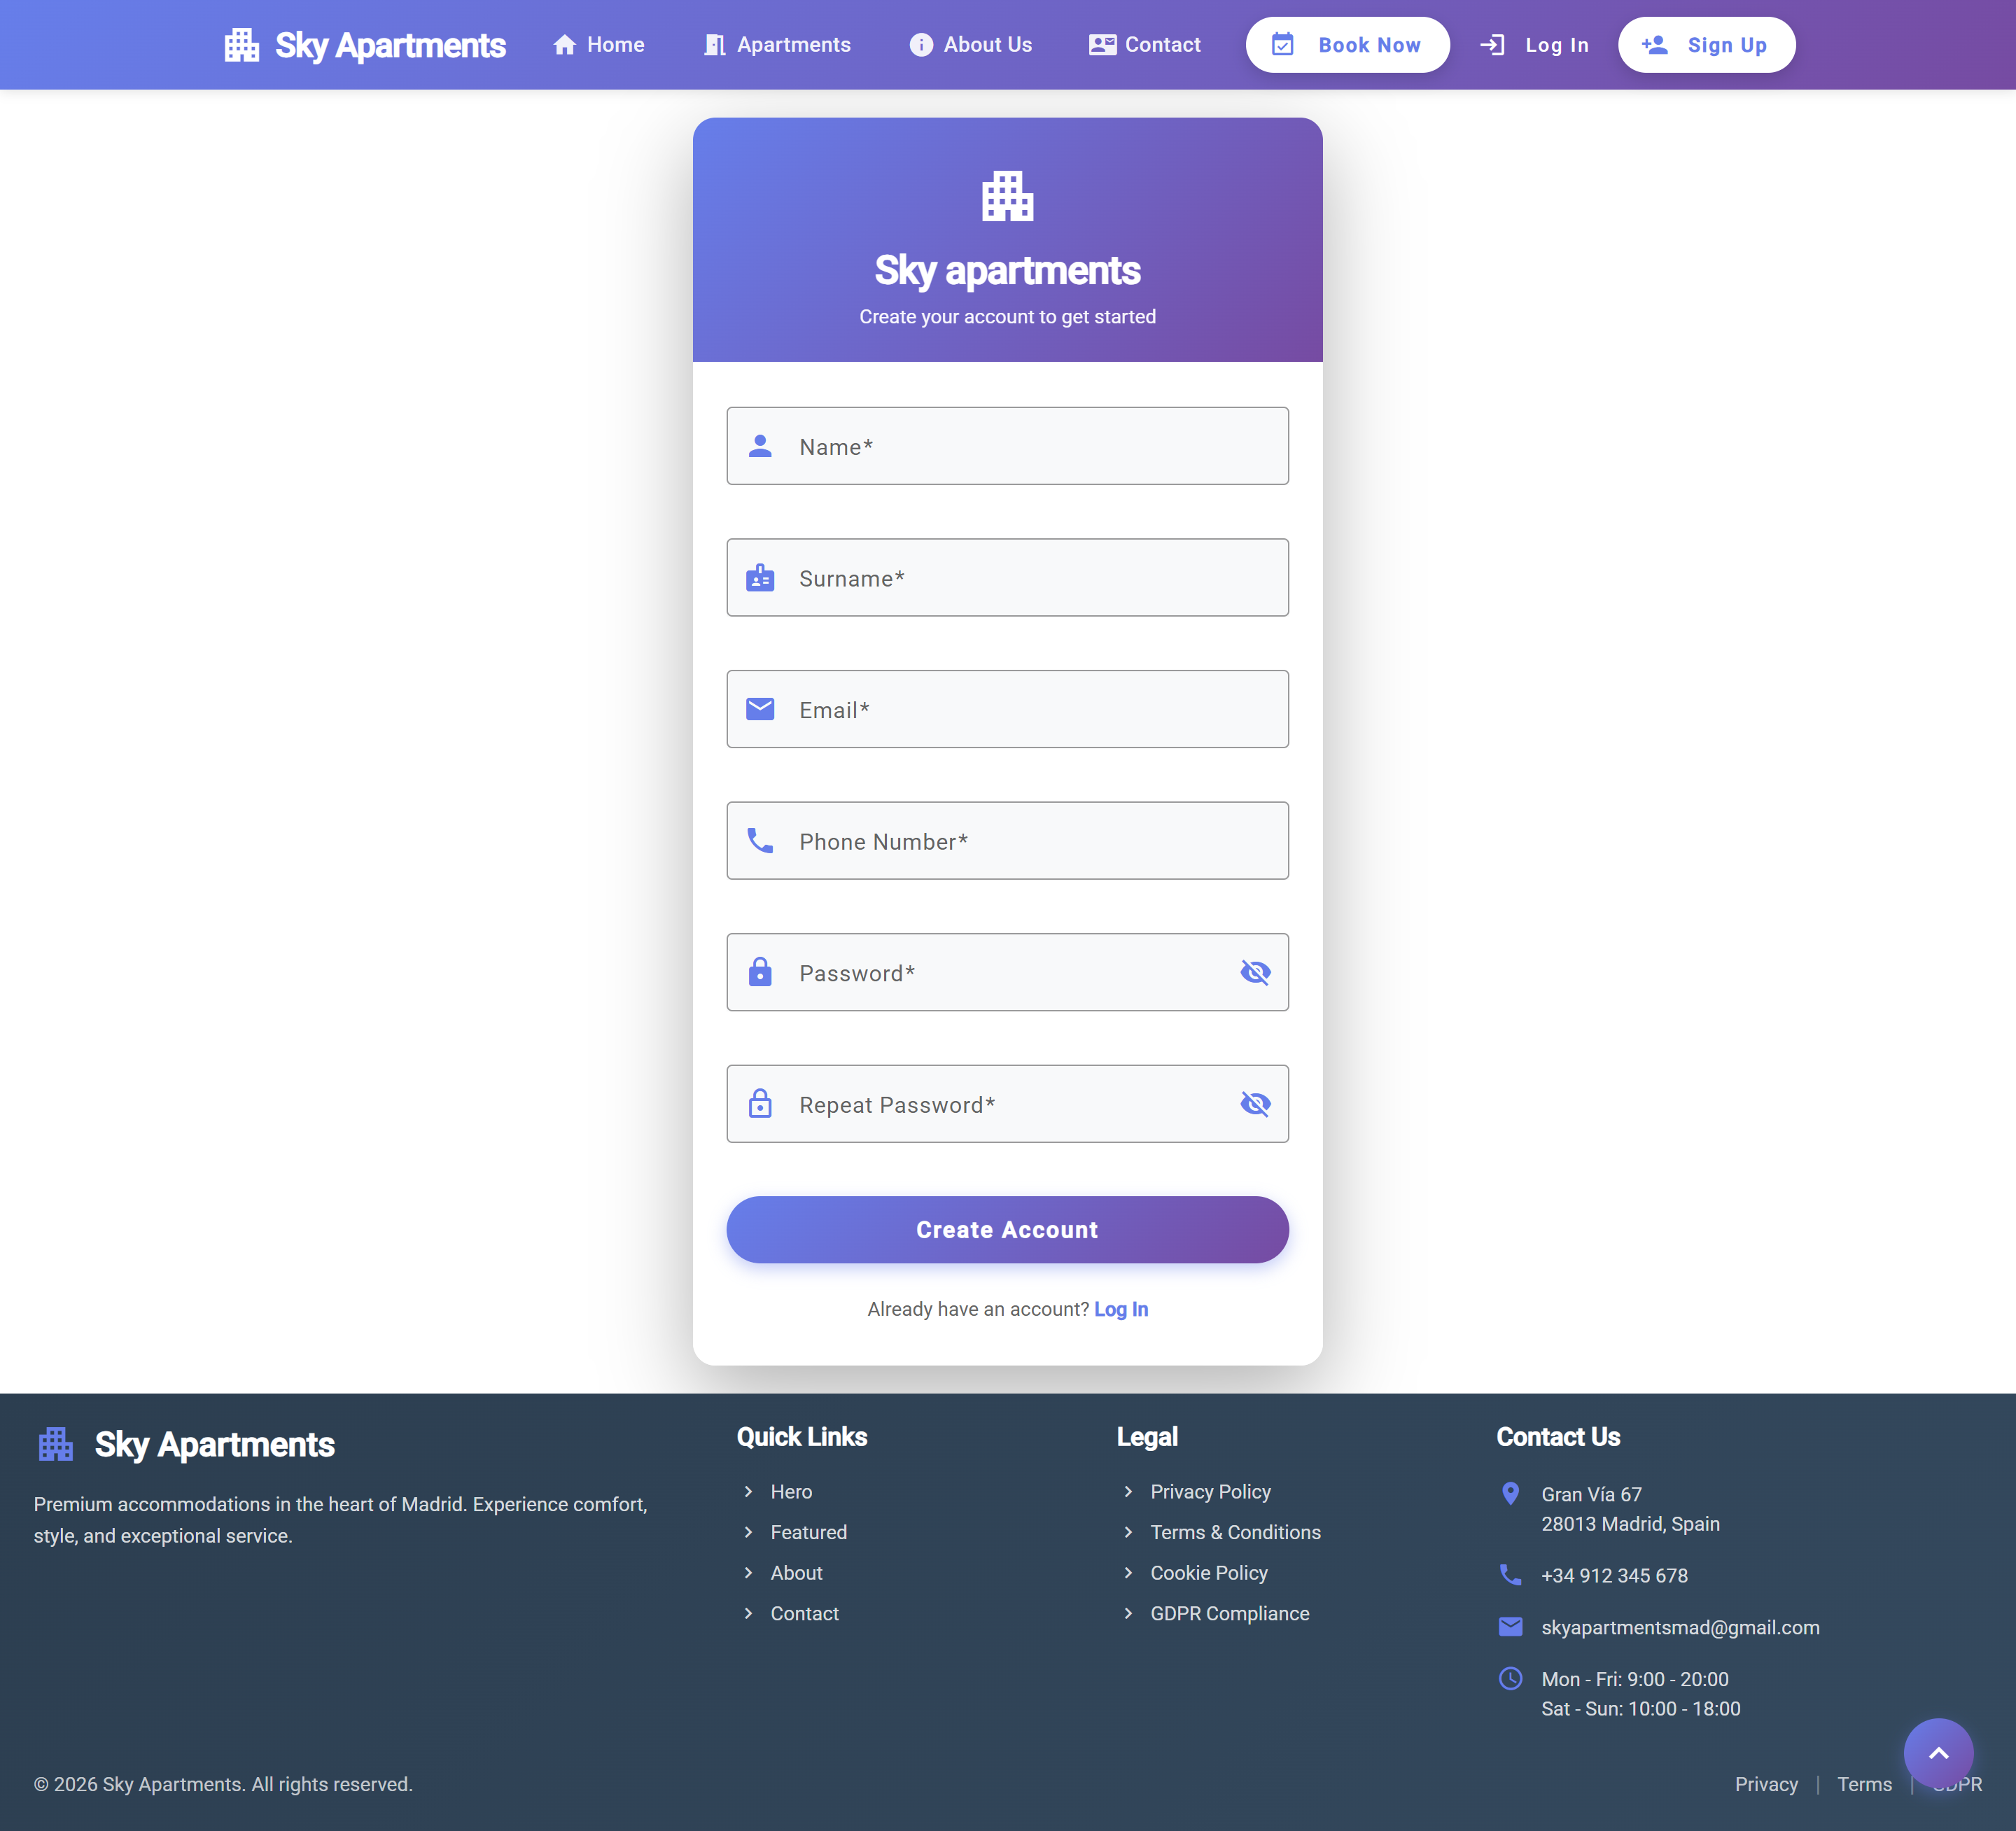
\includegraphics[width=0.8\textwidth]{img/screencapture-13-60-118-214-signup-2026-02-23-21_45_59.png}
    \caption{Formulario de registro para nuevos usuarios (Sign Up).}
\end{figure}

\begin{figure}[H]
    \centering
    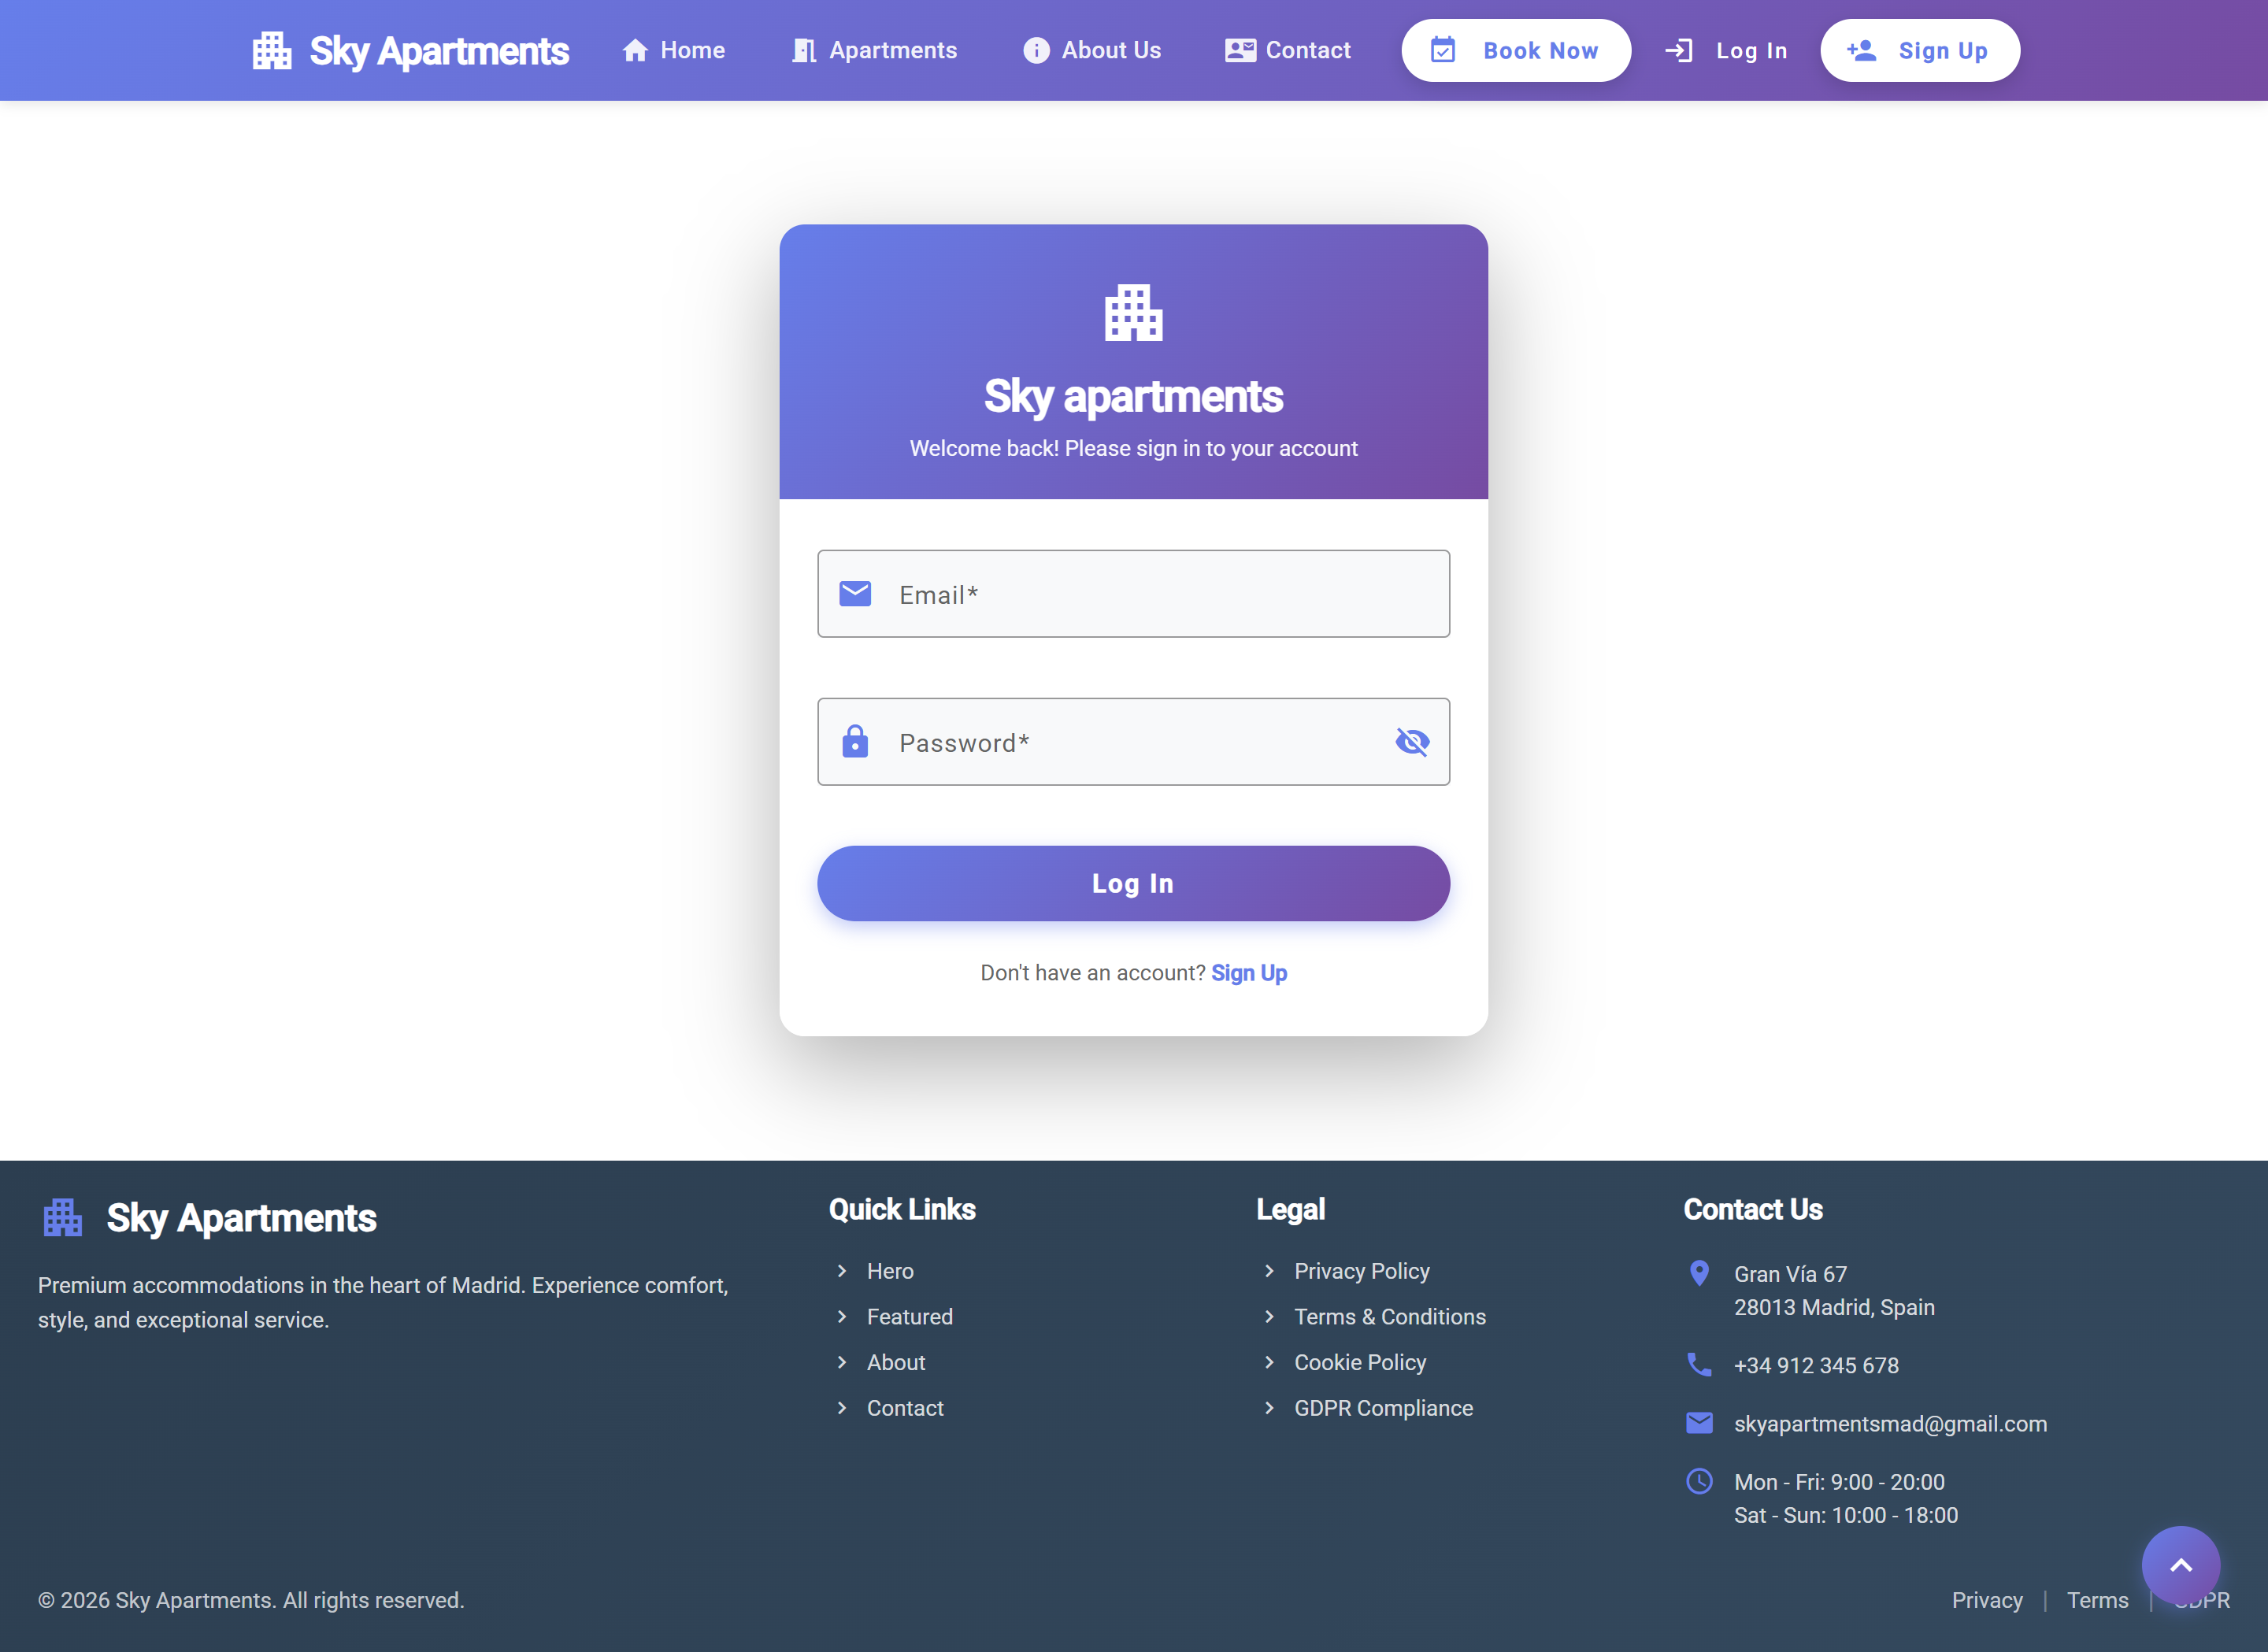
\includegraphics[width=0.8\textwidth]{img/screencapture-13-60-118-214-login-2026-02-23-21_45_52.png}
    \caption{Pantalla de inicio de sesión seguro (Log In).}
\end{figure}

\subsection{Explorando el Catálogo y Filtros}
En la sección principal de alojamientos, dispone de un buscador intuitivo en la barra lateral izquierda. Este panel permite filtrar los resultados en tiempo real basándose en sus necesidades: capacidad mínima (número de huéspedes), valoración media y comodidades requeridas (WiFi, piscina, terraza, etc.).

\begin{figure}[H]
    \centering
    \includegraphics[width=0.55\textwidth]{img/screencapture-13-60-118-214-apartments-2026-02-23-21_45_08.png}
    \caption{Catálogo de apartamentos con filtros avanzados en la barra lateral.}
\end{figure}

\subsection{Búsqueda por Fechas y Proceso de Reserva}
Si tiene unas fechas de viaje cerradas, puede hacer clic en el botón \textbf{"Book Now"}. Esto desplegará una interfaz específica donde podrá establecer las fechas exactas de \textit{Check-in} y \textit{Check-out}. El sistema calculará la disponibilidad en tiempo real y le mostrará únicamente las opciones libres.

\begin{figure}[H]
    \centering
    \includegraphics[width=0.55\textwidth]{img/screencapture-13-60-118-214-book-apartment-2026-02-23-21_45_24.png}
    \caption{Interfaz de selección de fechas para comprobar disponibilidad y calcular precios.}
\end{figure}

\subsection{Detalle del Apartamento y Reseñas}
Al seleccionar un alojamiento, accederá a su página de detalle. Aquí podrá explorar una galería interactiva de imágenes, leer la descripción y utilizar el widget lateral para confirmar la reserva. En la parte inferior, podrá leer las reseñas (de 1 a 5 estrellas) dejadas por huéspedes anteriores, así como escribir la suya propia tras finalizar su estancia.

\begin{figure}[H]
    \centering
    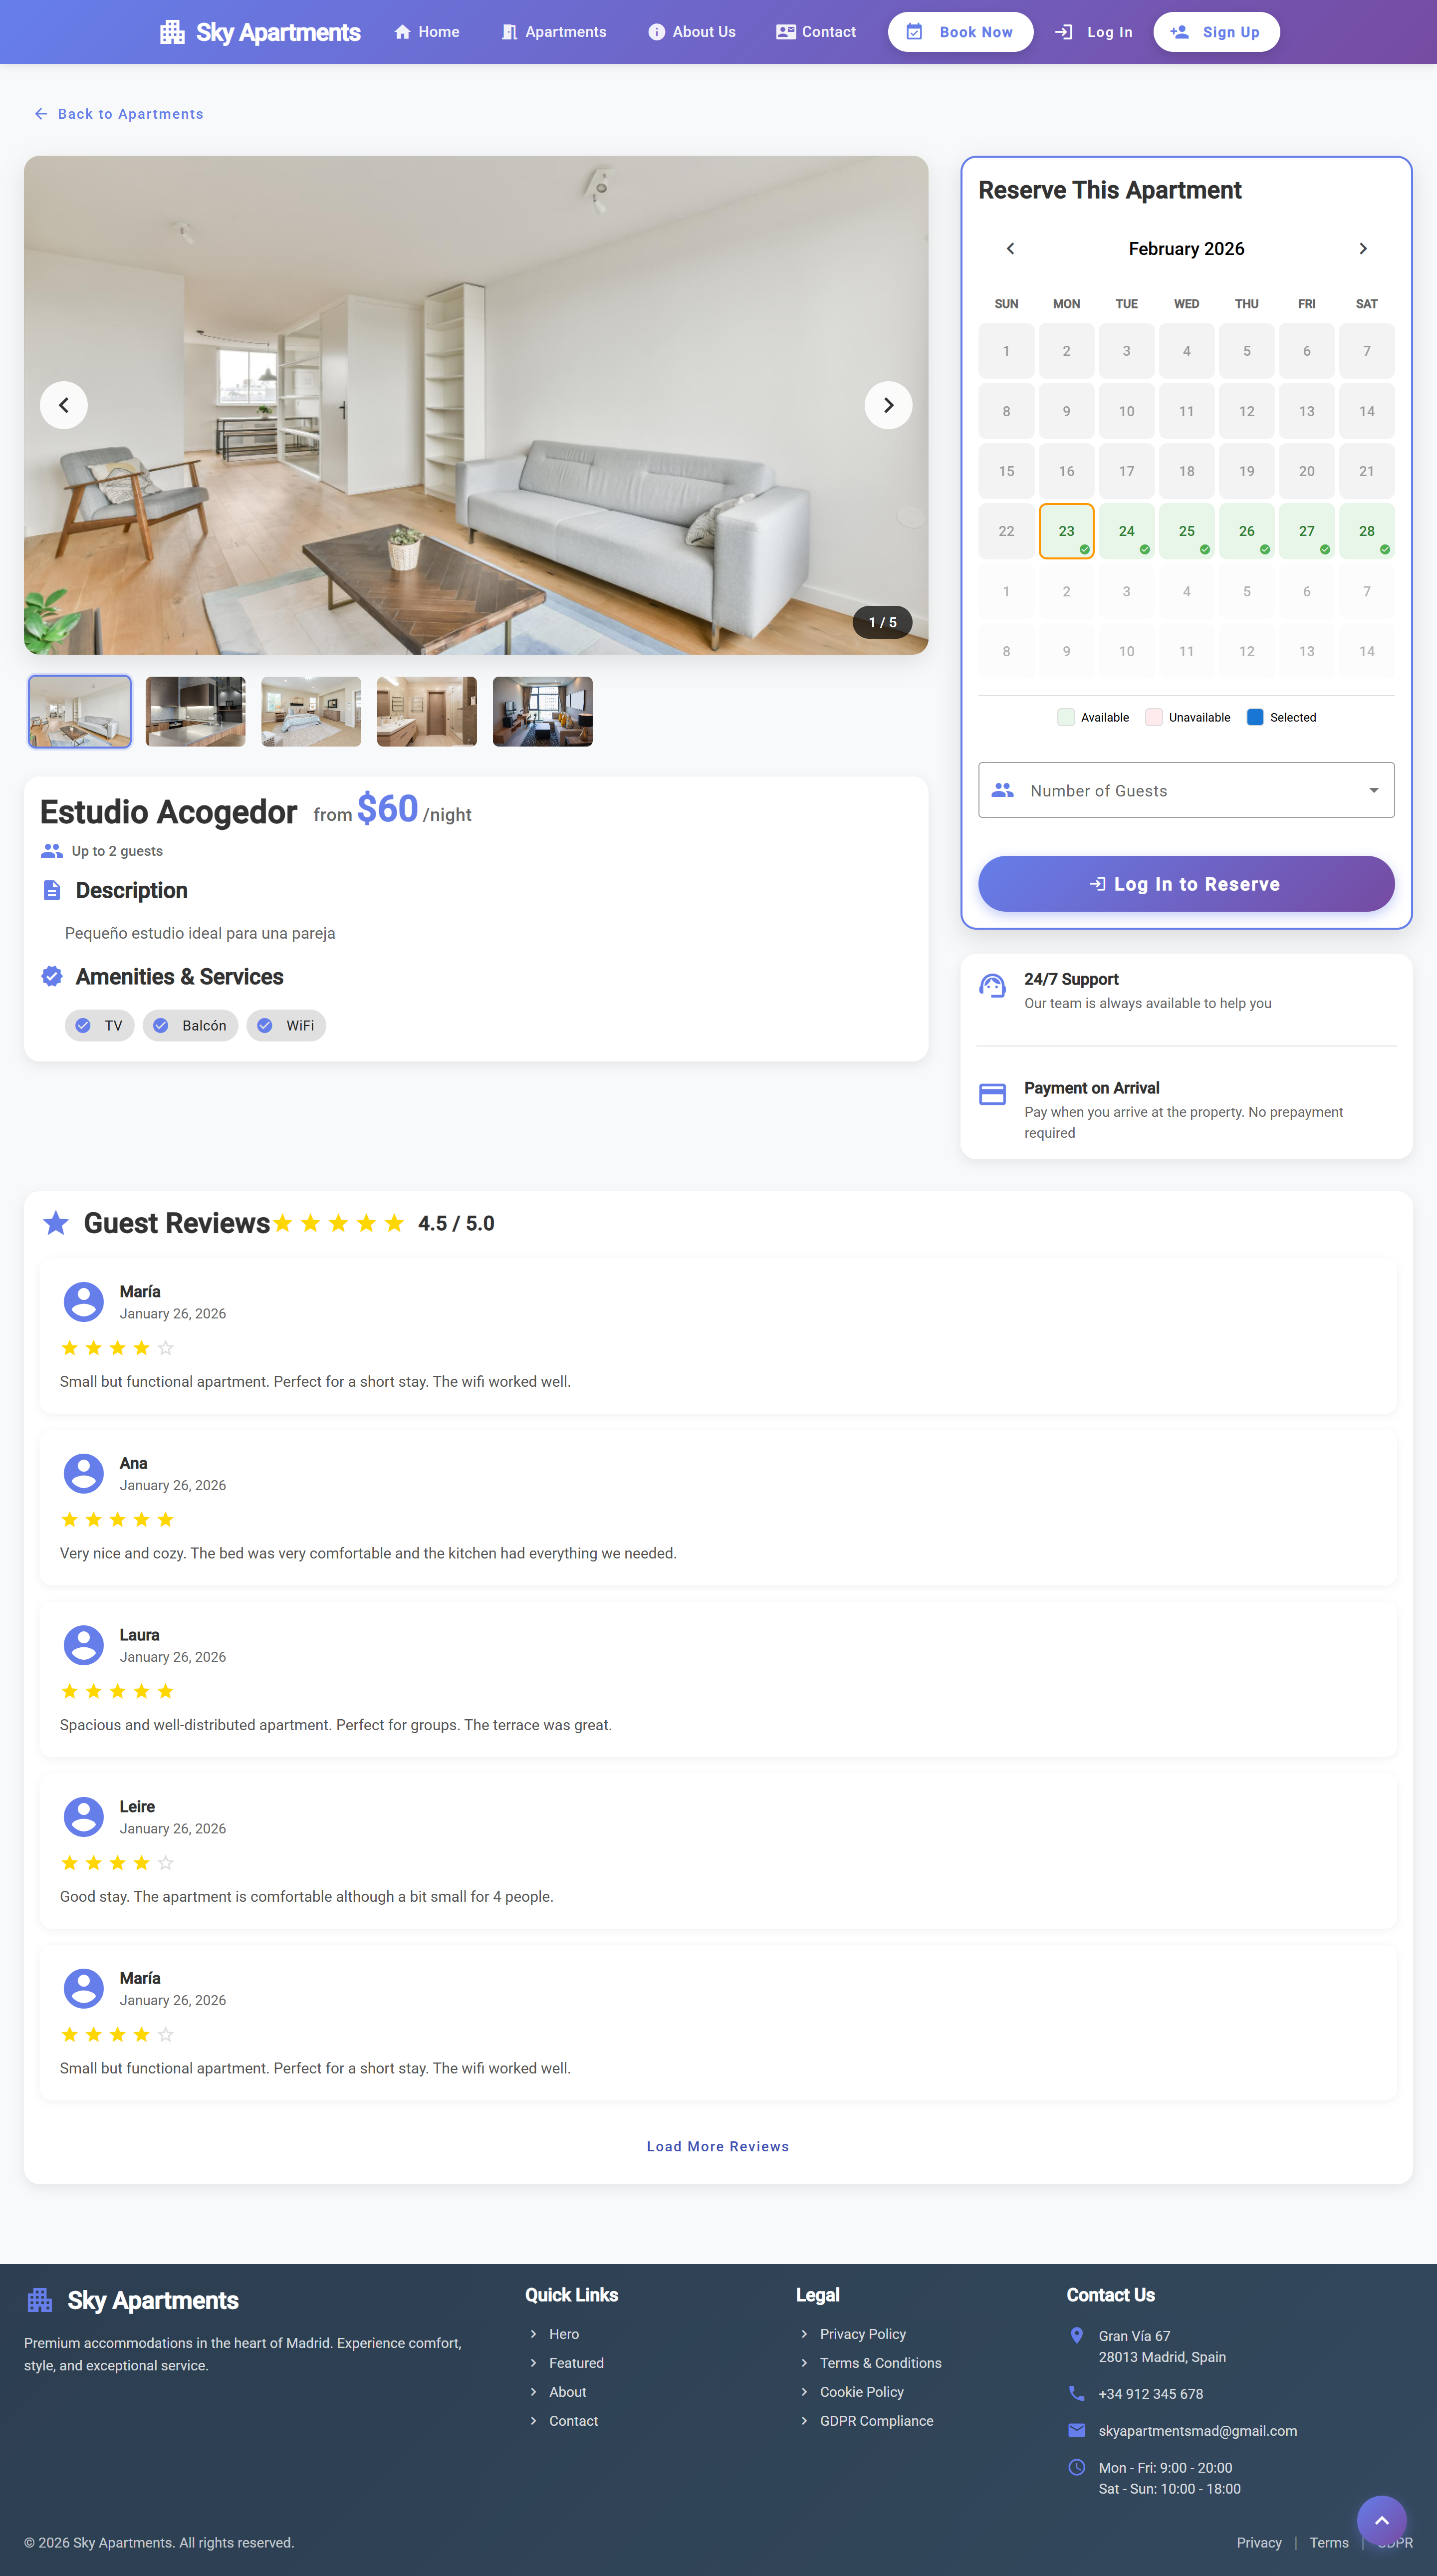
\includegraphics[width=0.8\textwidth]{img/screencapture-13-60-118-214-apartment-3-2026-02-23-21_45_42.png}
    \caption{Vista detallada de un apartamento, calendario de reservas y sistema de reseñas.}
\end{figure}

\subsection{Gestión de la Cuenta y Perfil Personal}
Haciendo clic en el icono de sus iniciales (esquina superior derecha), accederá a su área personal. En la pestaña \textbf{"Personal Information"} podrá consultar y actualizar sus datos de contacto en cualquier momento, así como modificar su contraseña de acceso.

\begin{figure}[H]
    \centering
    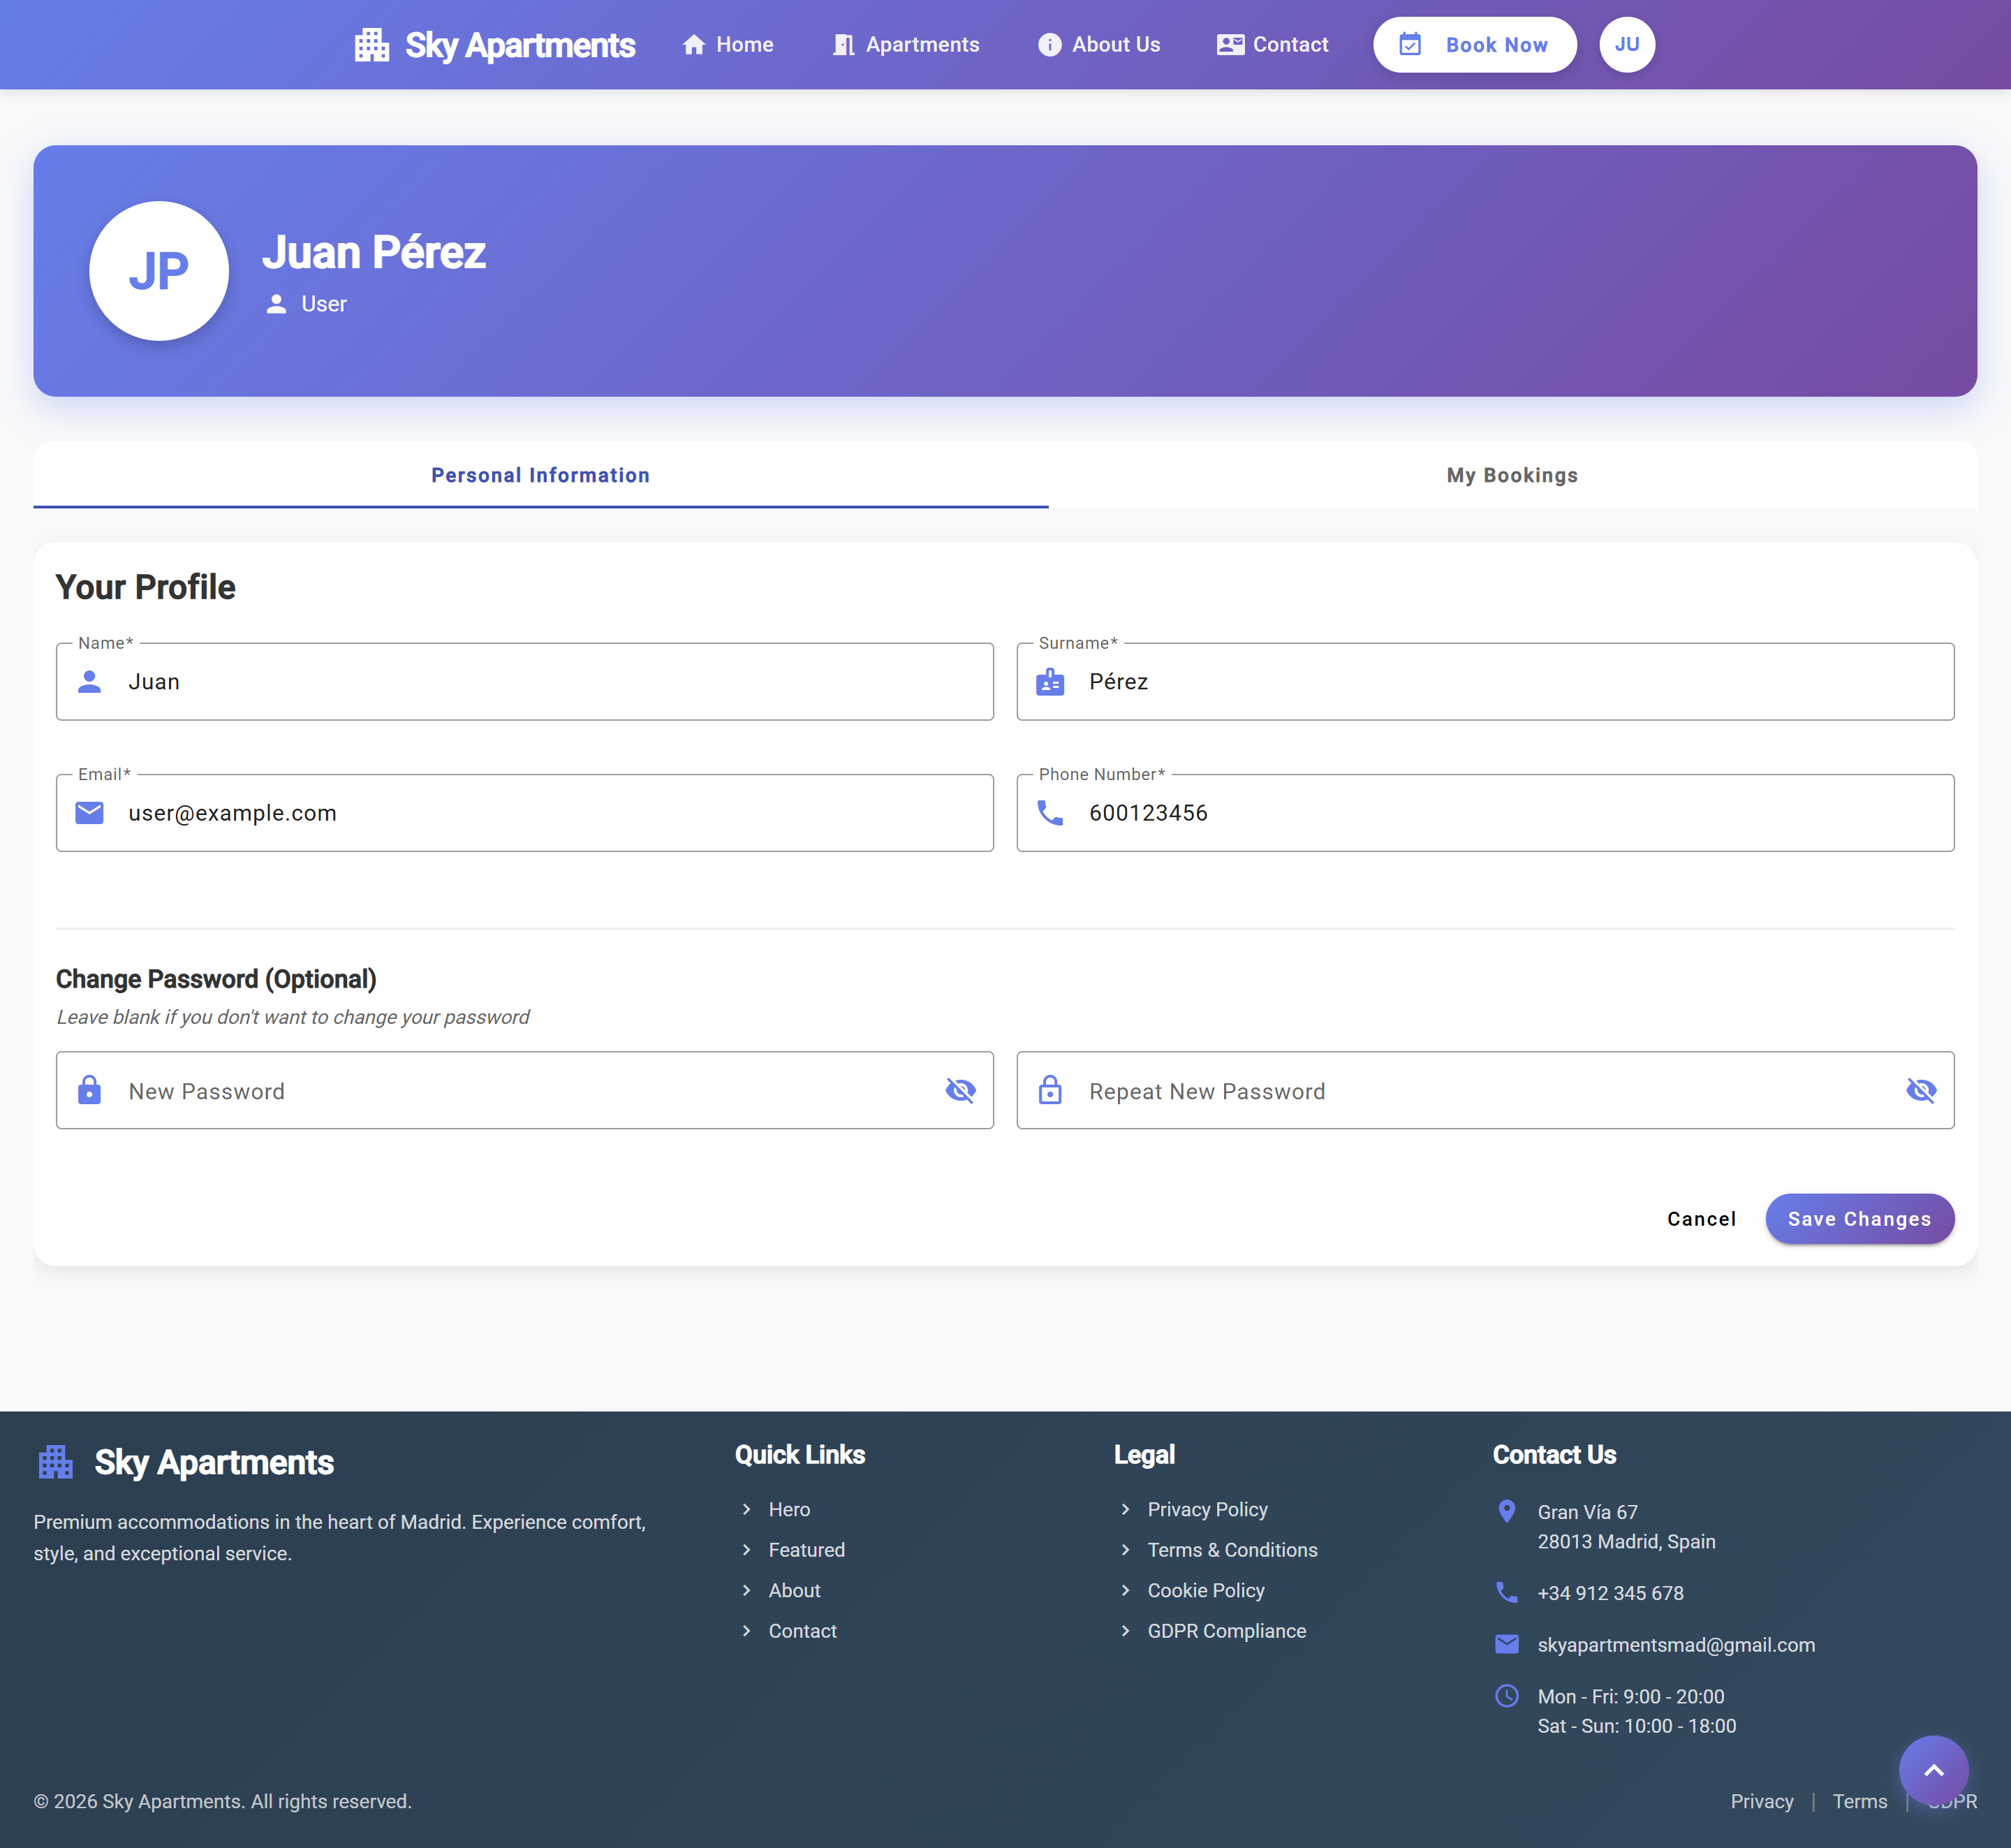
\includegraphics[width=0.8\textwidth]{img/screencapture-13-60-118-214-profile-2026-02-23-21_46_26.png}
    \caption{Área de gestión de datos personales del perfil de usuario.}
\end{figure}

En la pestaña \textbf{"My Bookings"} (Mis Reservas), podrá consultar su historial completo, ver el estado de cada estancia (confirmada, completada, cancelada) y cancelar activamente aquellas reservas que aún no hayan comenzado.

\begin{figure}[H]
    \centering
    \includegraphics[width=0.6\textwidth]{img/screencapture-13-60-118-214-profile-2026-02-23-21_46_40.png}
    \caption{Historial de reservas del usuario y gestión de cancelaciones.}
\end{figure}


\section{Guía de Administración (Panel Privado)}
Los usuarios con el rol de Administrador tienen acceso a un panel de control avanzado desde donde pueden gestionar integralmente el negocio.

\subsection{Dashboard Analítico}
Al entrar al panel, la pestaña \textbf{"Dashboard"} ofrece una visión panorámica del rendimiento. Incluye métricas clave como los ingresos totales generados, una gráfica de la ocupación en el tiempo y ránkings automáticos de los apartamentos más reservados y los mejor valorados. Esta información se puede filtrar por períodos específicos para analizar tendencias estacionales o el impacto de promociones.

\begin{figure}[H]
    \centering
    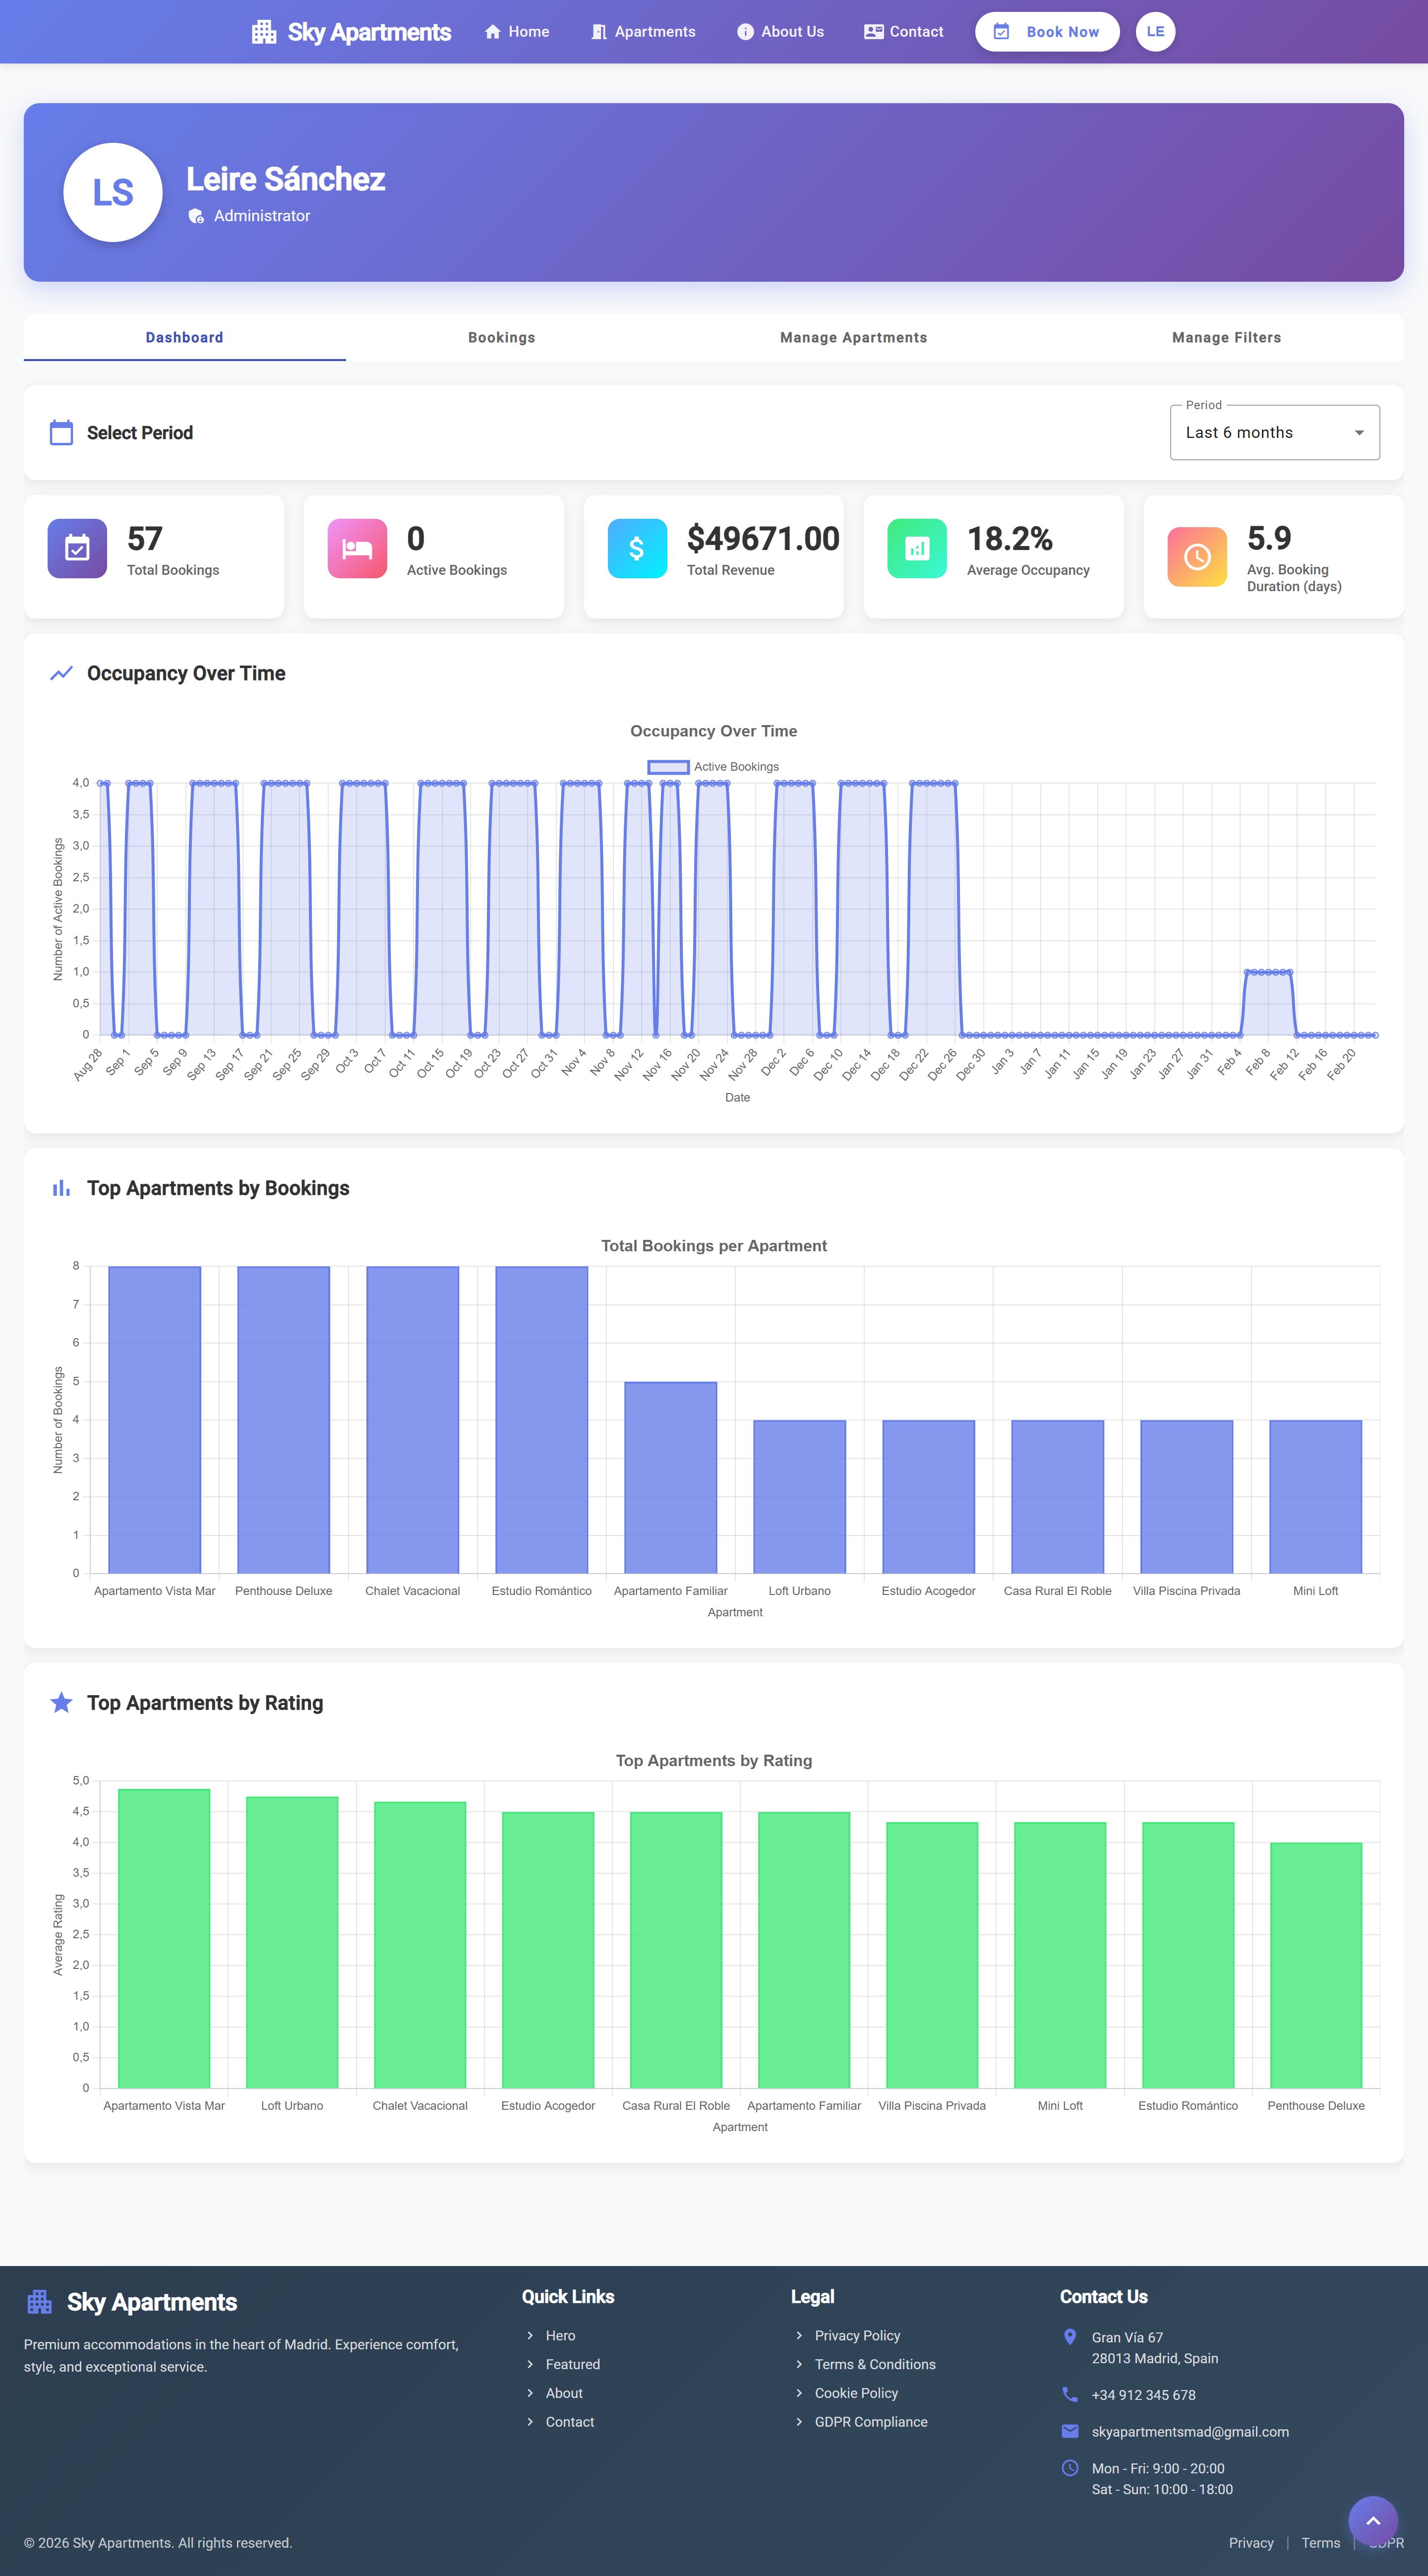
\includegraphics[width=0.8\textwidth]{img/screencapture-13-60-118-214-profile-2026-02-23-21_47_11.png}
    \caption{Dashboard principal de administración con métricas y gráficas de rendimiento.}
\end{figure}

\subsection{Gestión Global de Reservas}
La pestaña \textbf{"Bookings"} permite al administrador supervisar toda la actividad. Ofrece una vista visual de calendario o formato lista, e incorpora un buscador y un filtro por estado para encontrar rápidamente reservas concretas, facilitando la gestión operativa.

\begin{figure}[H]
    \centering
    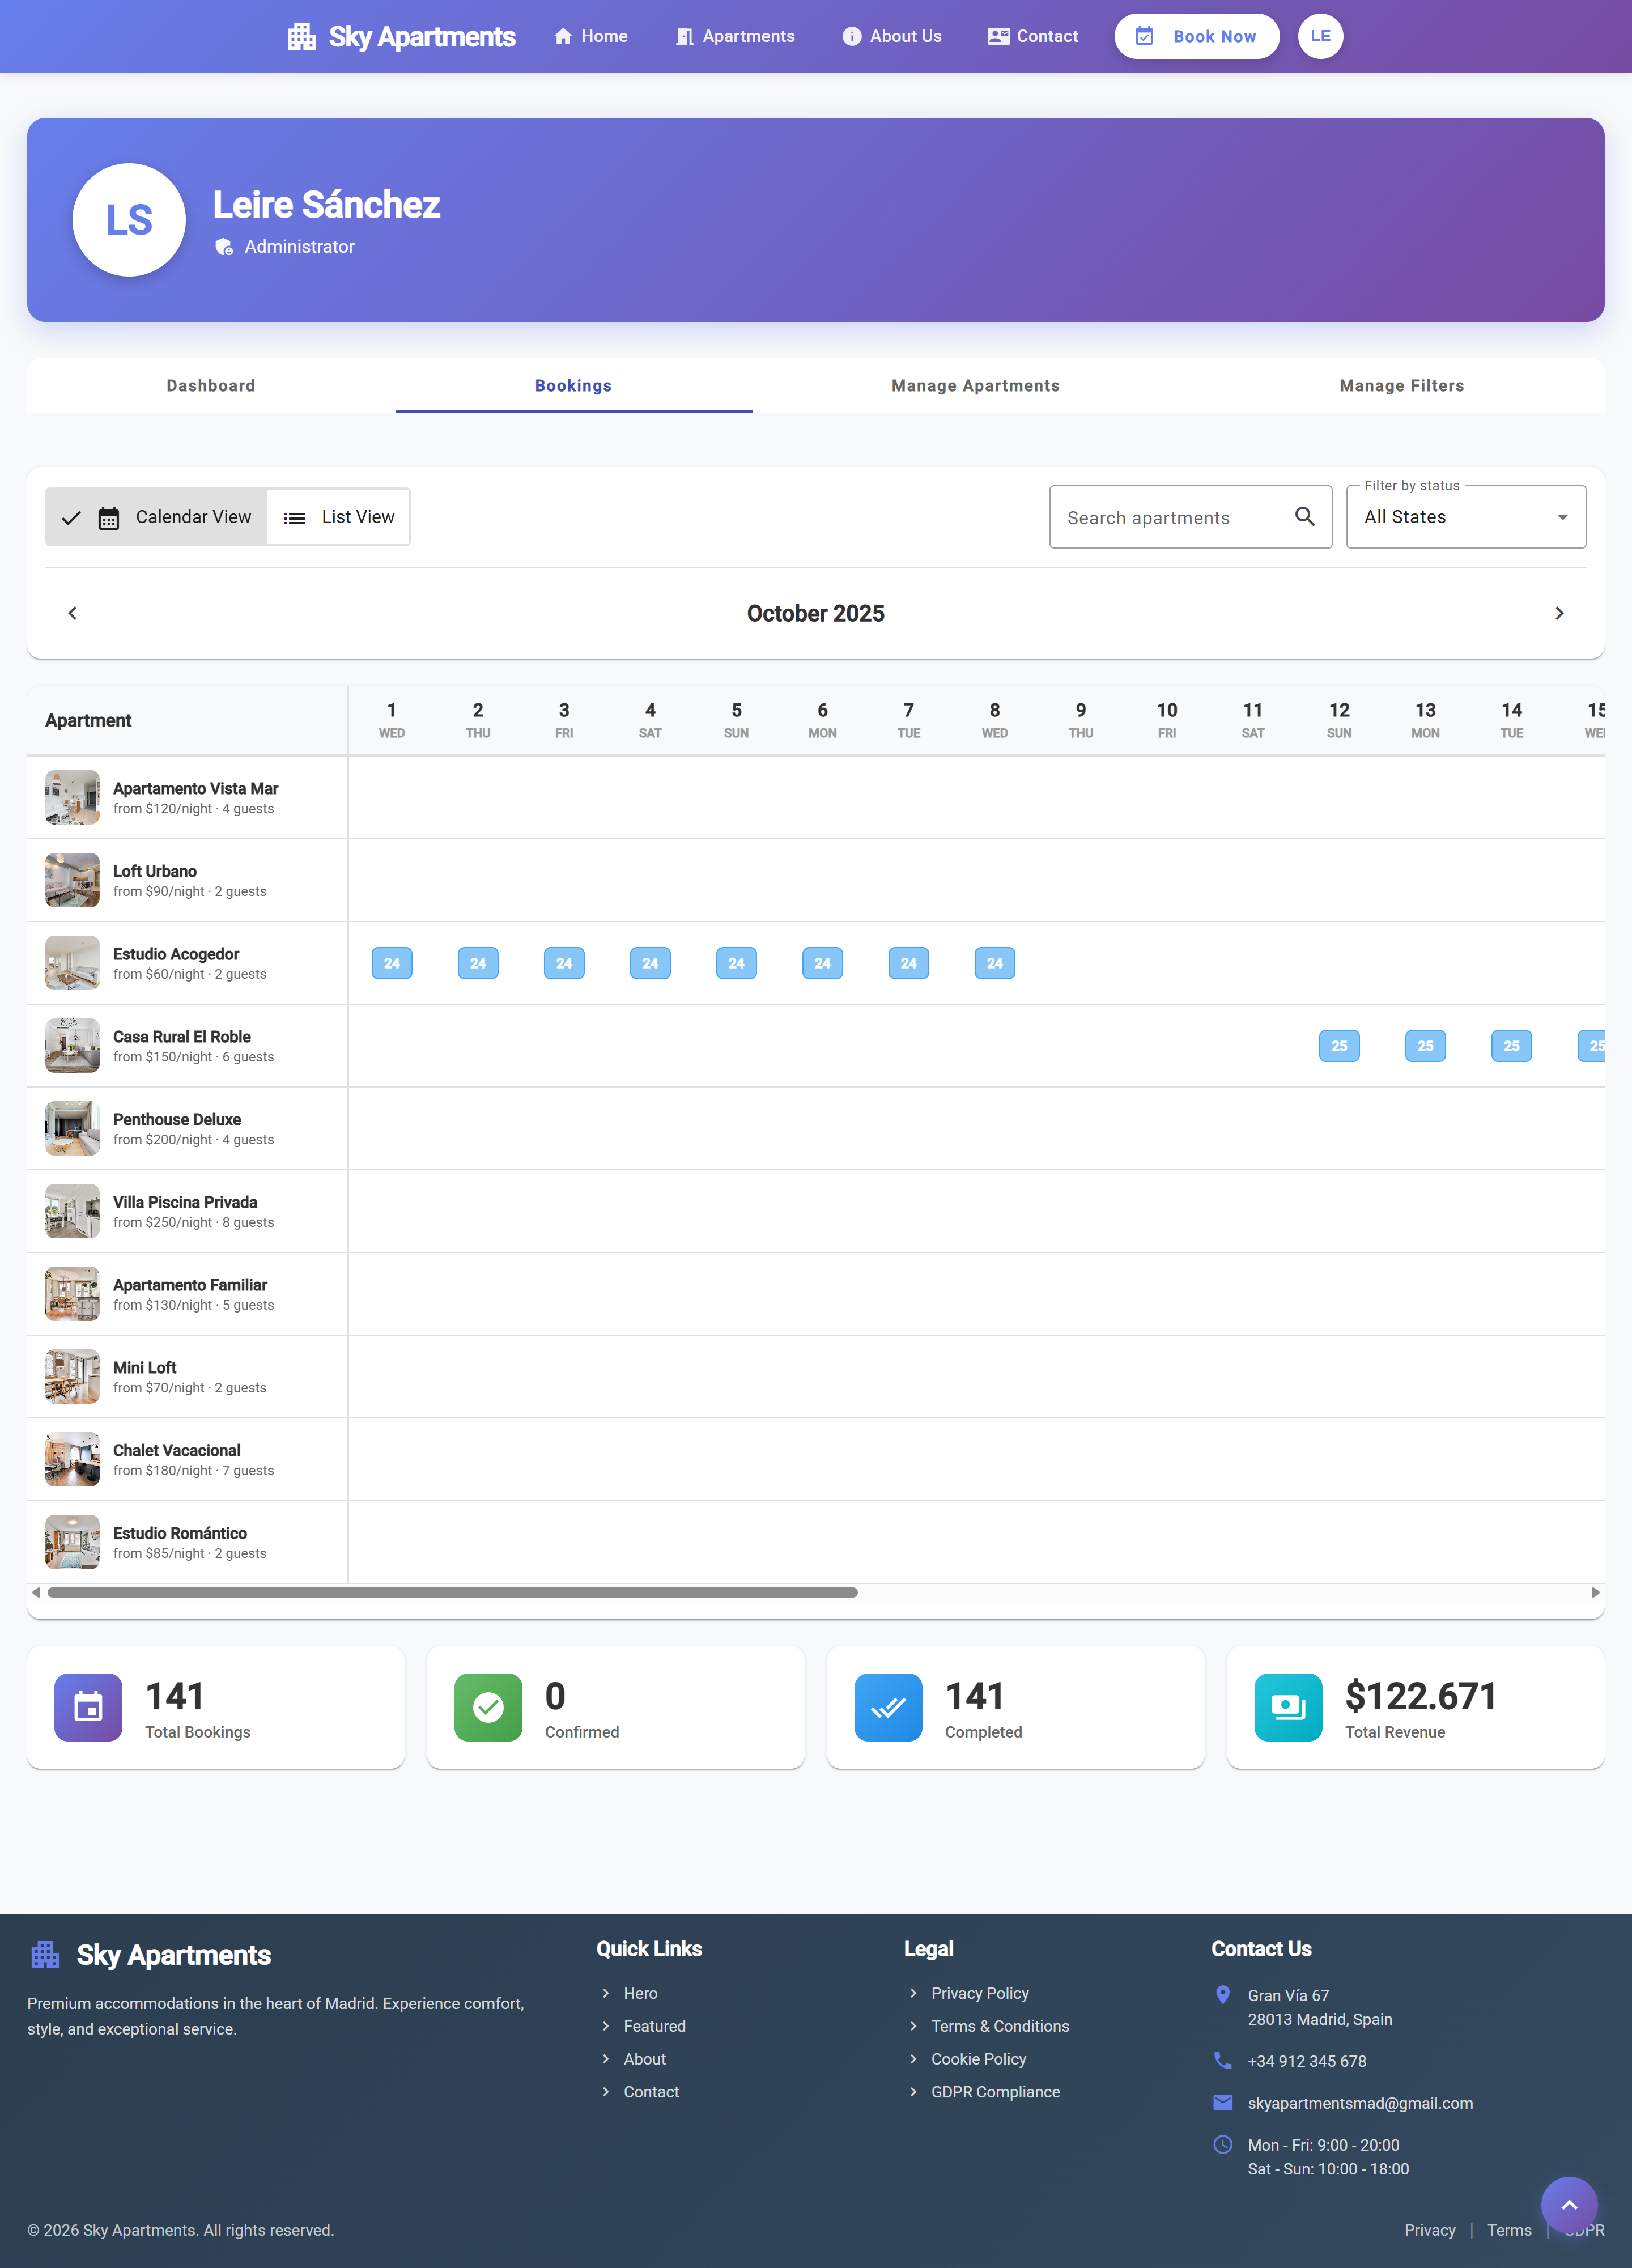
\includegraphics[width=0.8\textwidth]{img/screencapture-13-60-118-214-profile-2026-02-23-21_47_49.png}
    \caption{Panel de gestión y visualización de todas las reservas del sistema.}
\end{figure}

\subsection{Gestión del Catálogo de Apartamentos}
Desde la pestaña \textbf{"Manage Apartments"}, el administrador tiene una vista global de todos los alojamientos activos en el sistema, pudiendo editarlos o darlos de baja directamente desde sus respectivas tarjetas.

\begin{figure}[H]
    \centering
    \includegraphics[width=0.8\textwidth]{img/screencapture-13-60-118-214-profile-2026-02-23-21_48_01.png}
    \caption{Vista general del catálogo de alojamientos desde el panel de administración.}
\end{figure}

Haciendo clic en "Add Apartment", se abre un formulario para introducir todos los detalles de una nueva propiedad (nombre, capacidad, precio base, servicios) y subir de forma simultánea múltiples imágenes que conformarán su galería pública.

\begin{figure}[H]
    \centering
    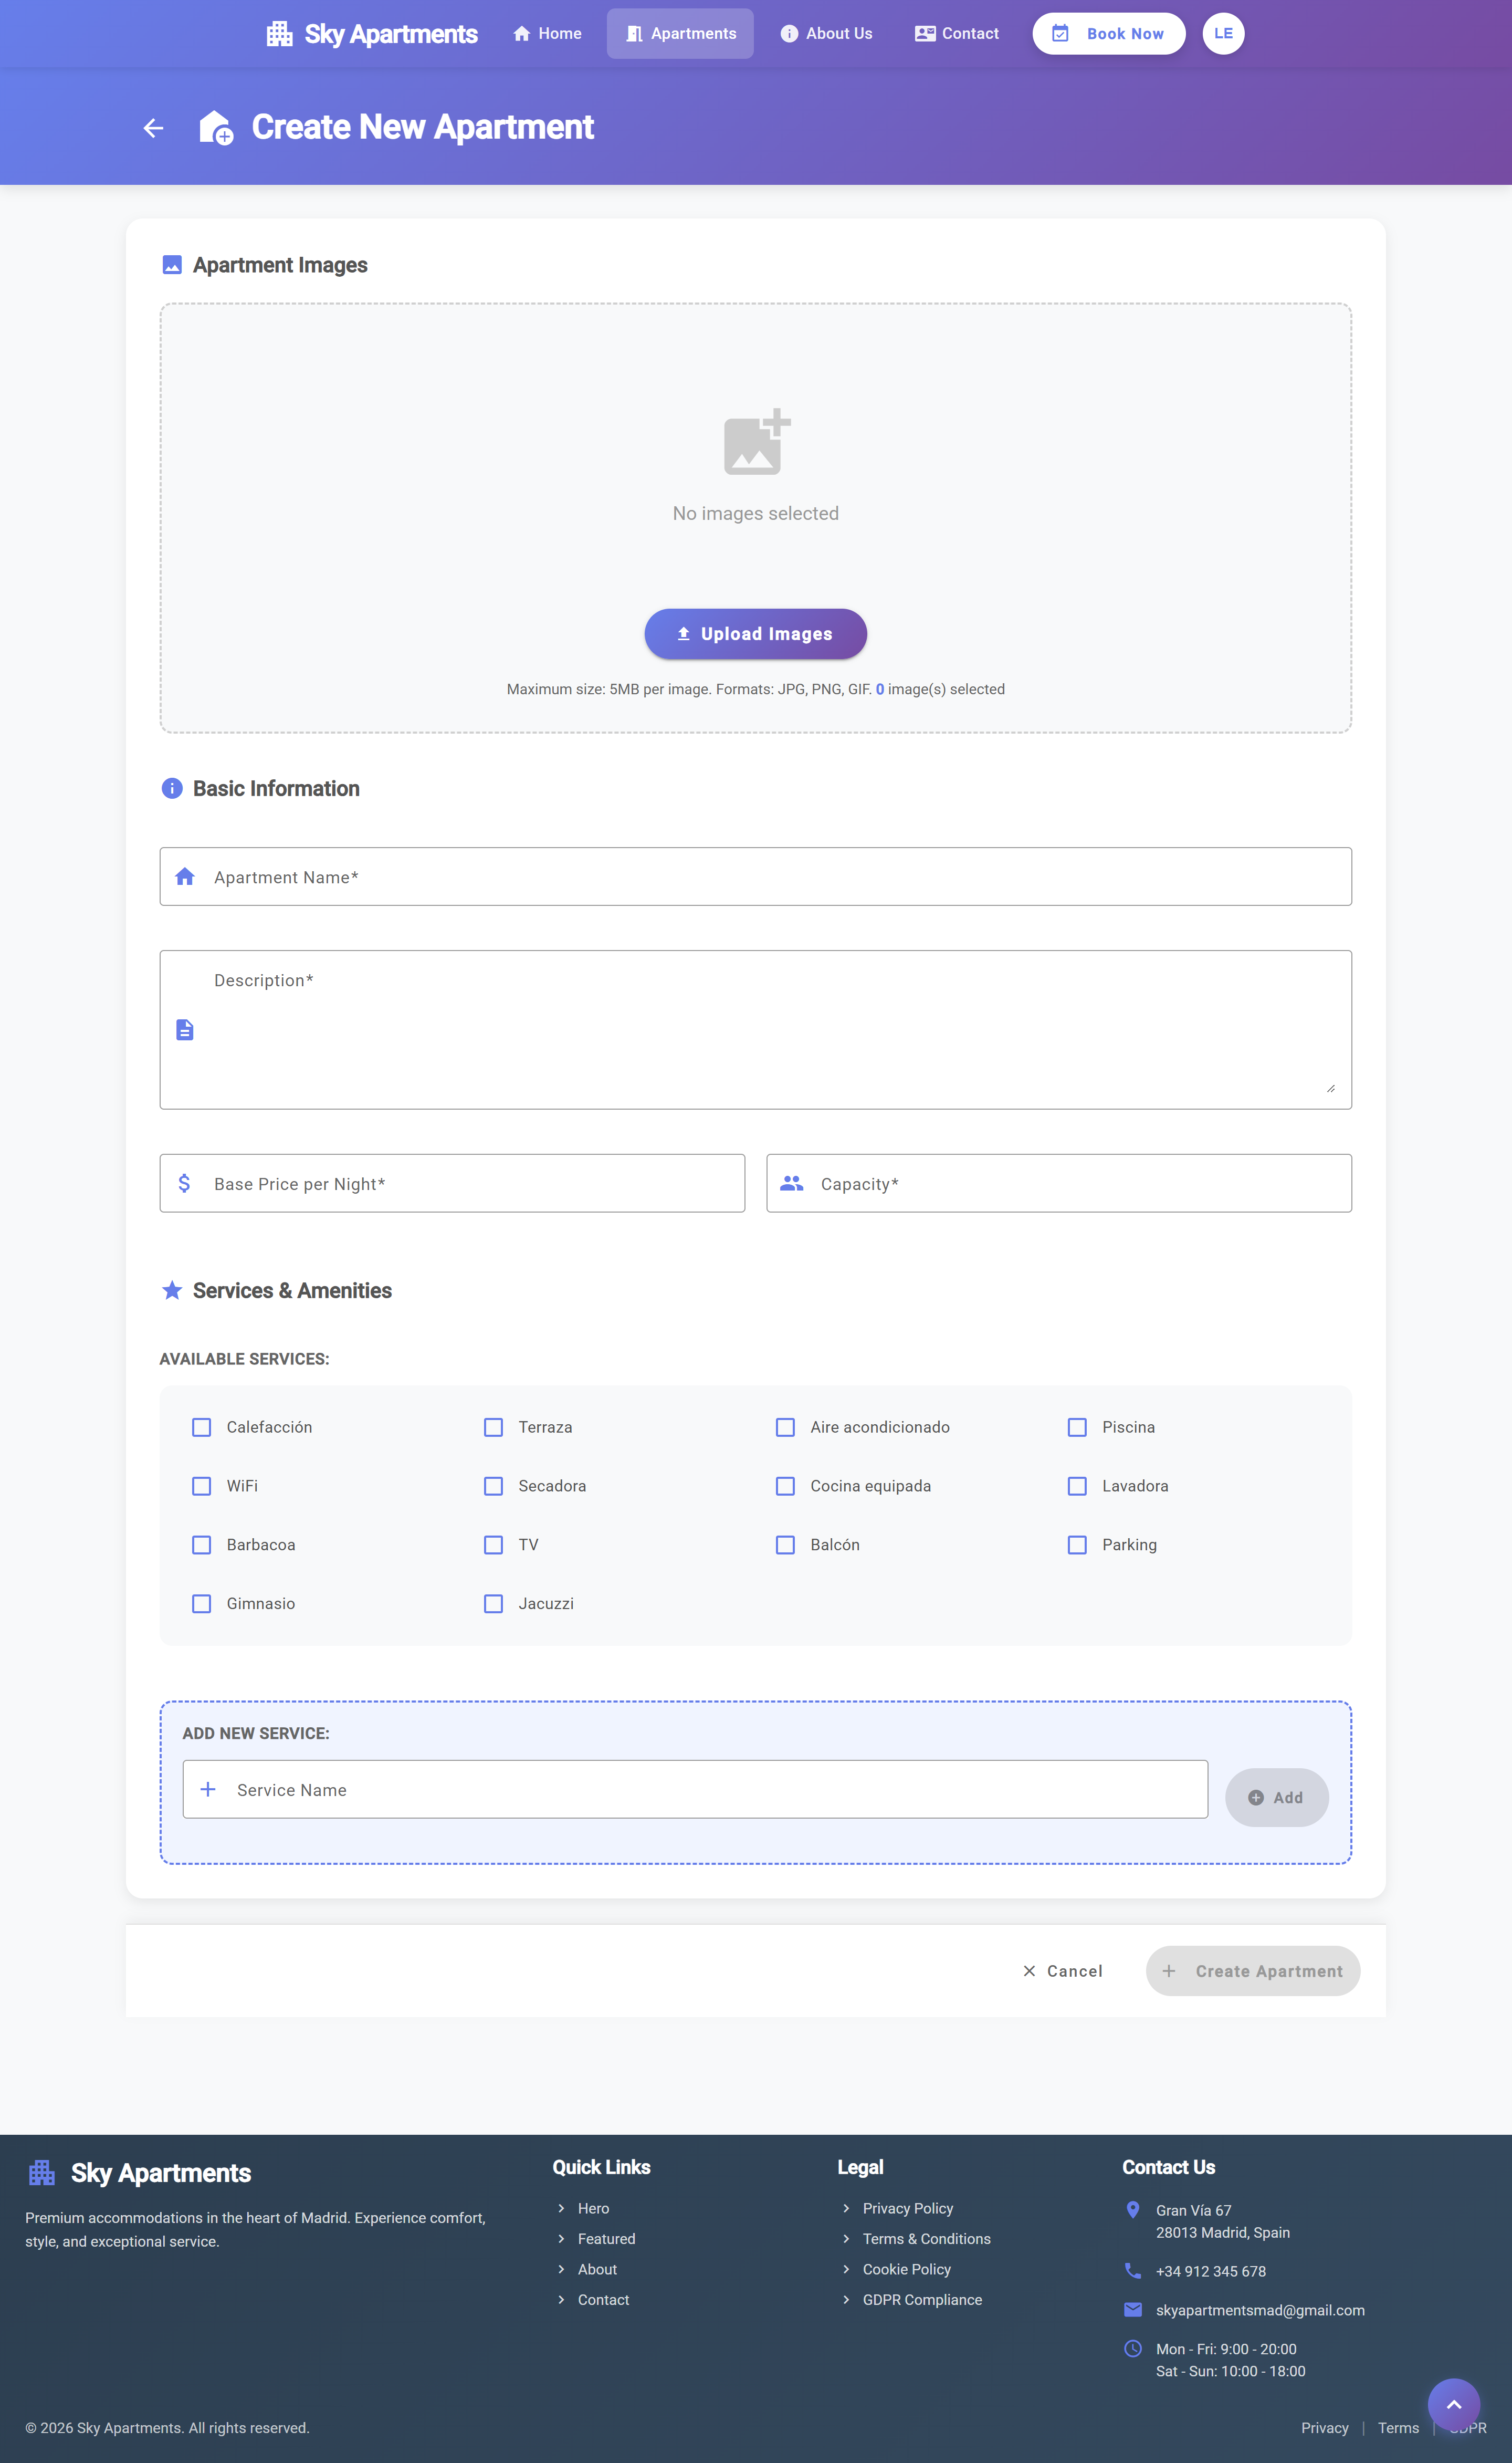
\includegraphics[width=0.8\textwidth]{img/screencapture-13-60-118-214-apartments-new-2026-02-23-21_48_14.png}
    \caption{Formulario de alta de un nuevo apartamento y subida de imágenes.}
\end{figure}

\subsection{Configuración de Precios Dinámicos (Filtros)}
La pestaña \textbf{"Manage Filters"} es el núcleo de la estrategia de ingresos. Aquí, el administrador puede visualizar, editar o eliminar todas las reglas de precio activas en la plataforma.

\begin{figure}[H]
    \centering
    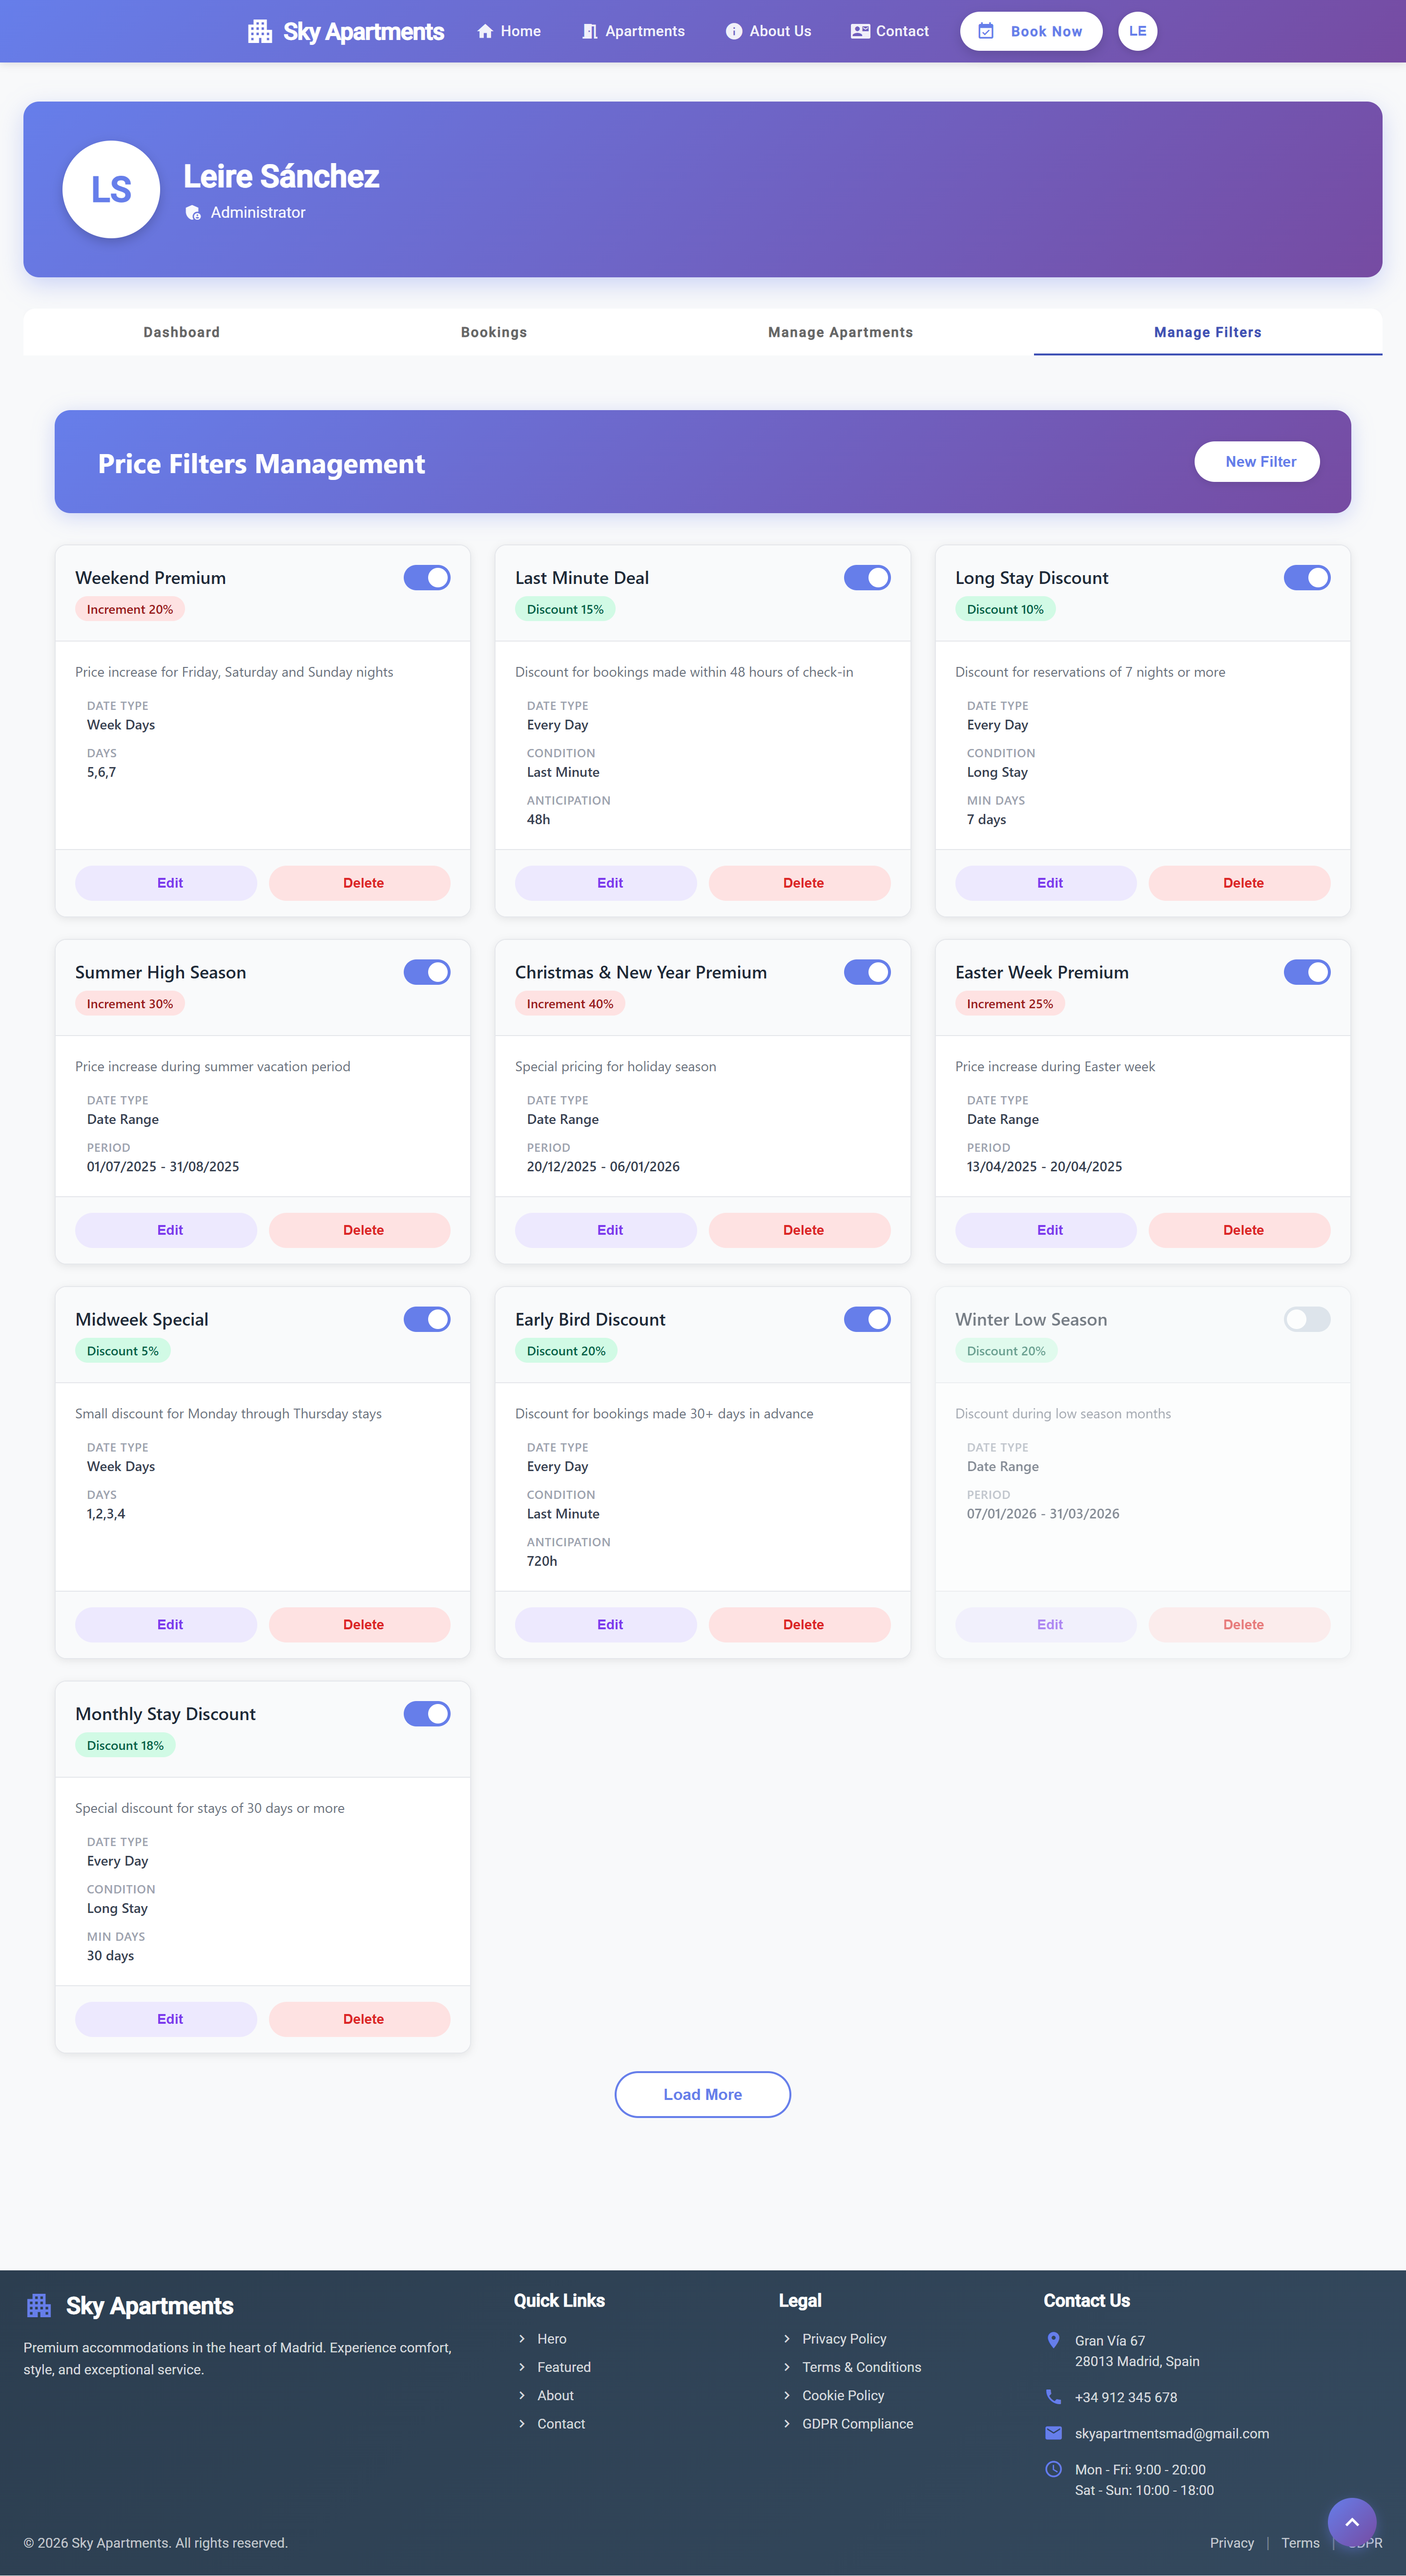
\includegraphics[width=0.8\textwidth]{img/screencapture-13-60-118-214-profile-2026-02-23-21_48_35.png}
    \caption{Listado de reglas y filtros de precios dinámicos configurados en el sistema.}
\end{figure}

Mediante el botón "New Filter", se despliega un modal avanzado que permite crear nuevas reglas. Se pueden configurar incrementos o descuentos porcentuales aplicables a rangos de fechas (temporadas), días de la semana (fines de semana), o condiciones especiales como reservas anticipadas y estancias largas.

\begin{figure}[H]
    \centering
    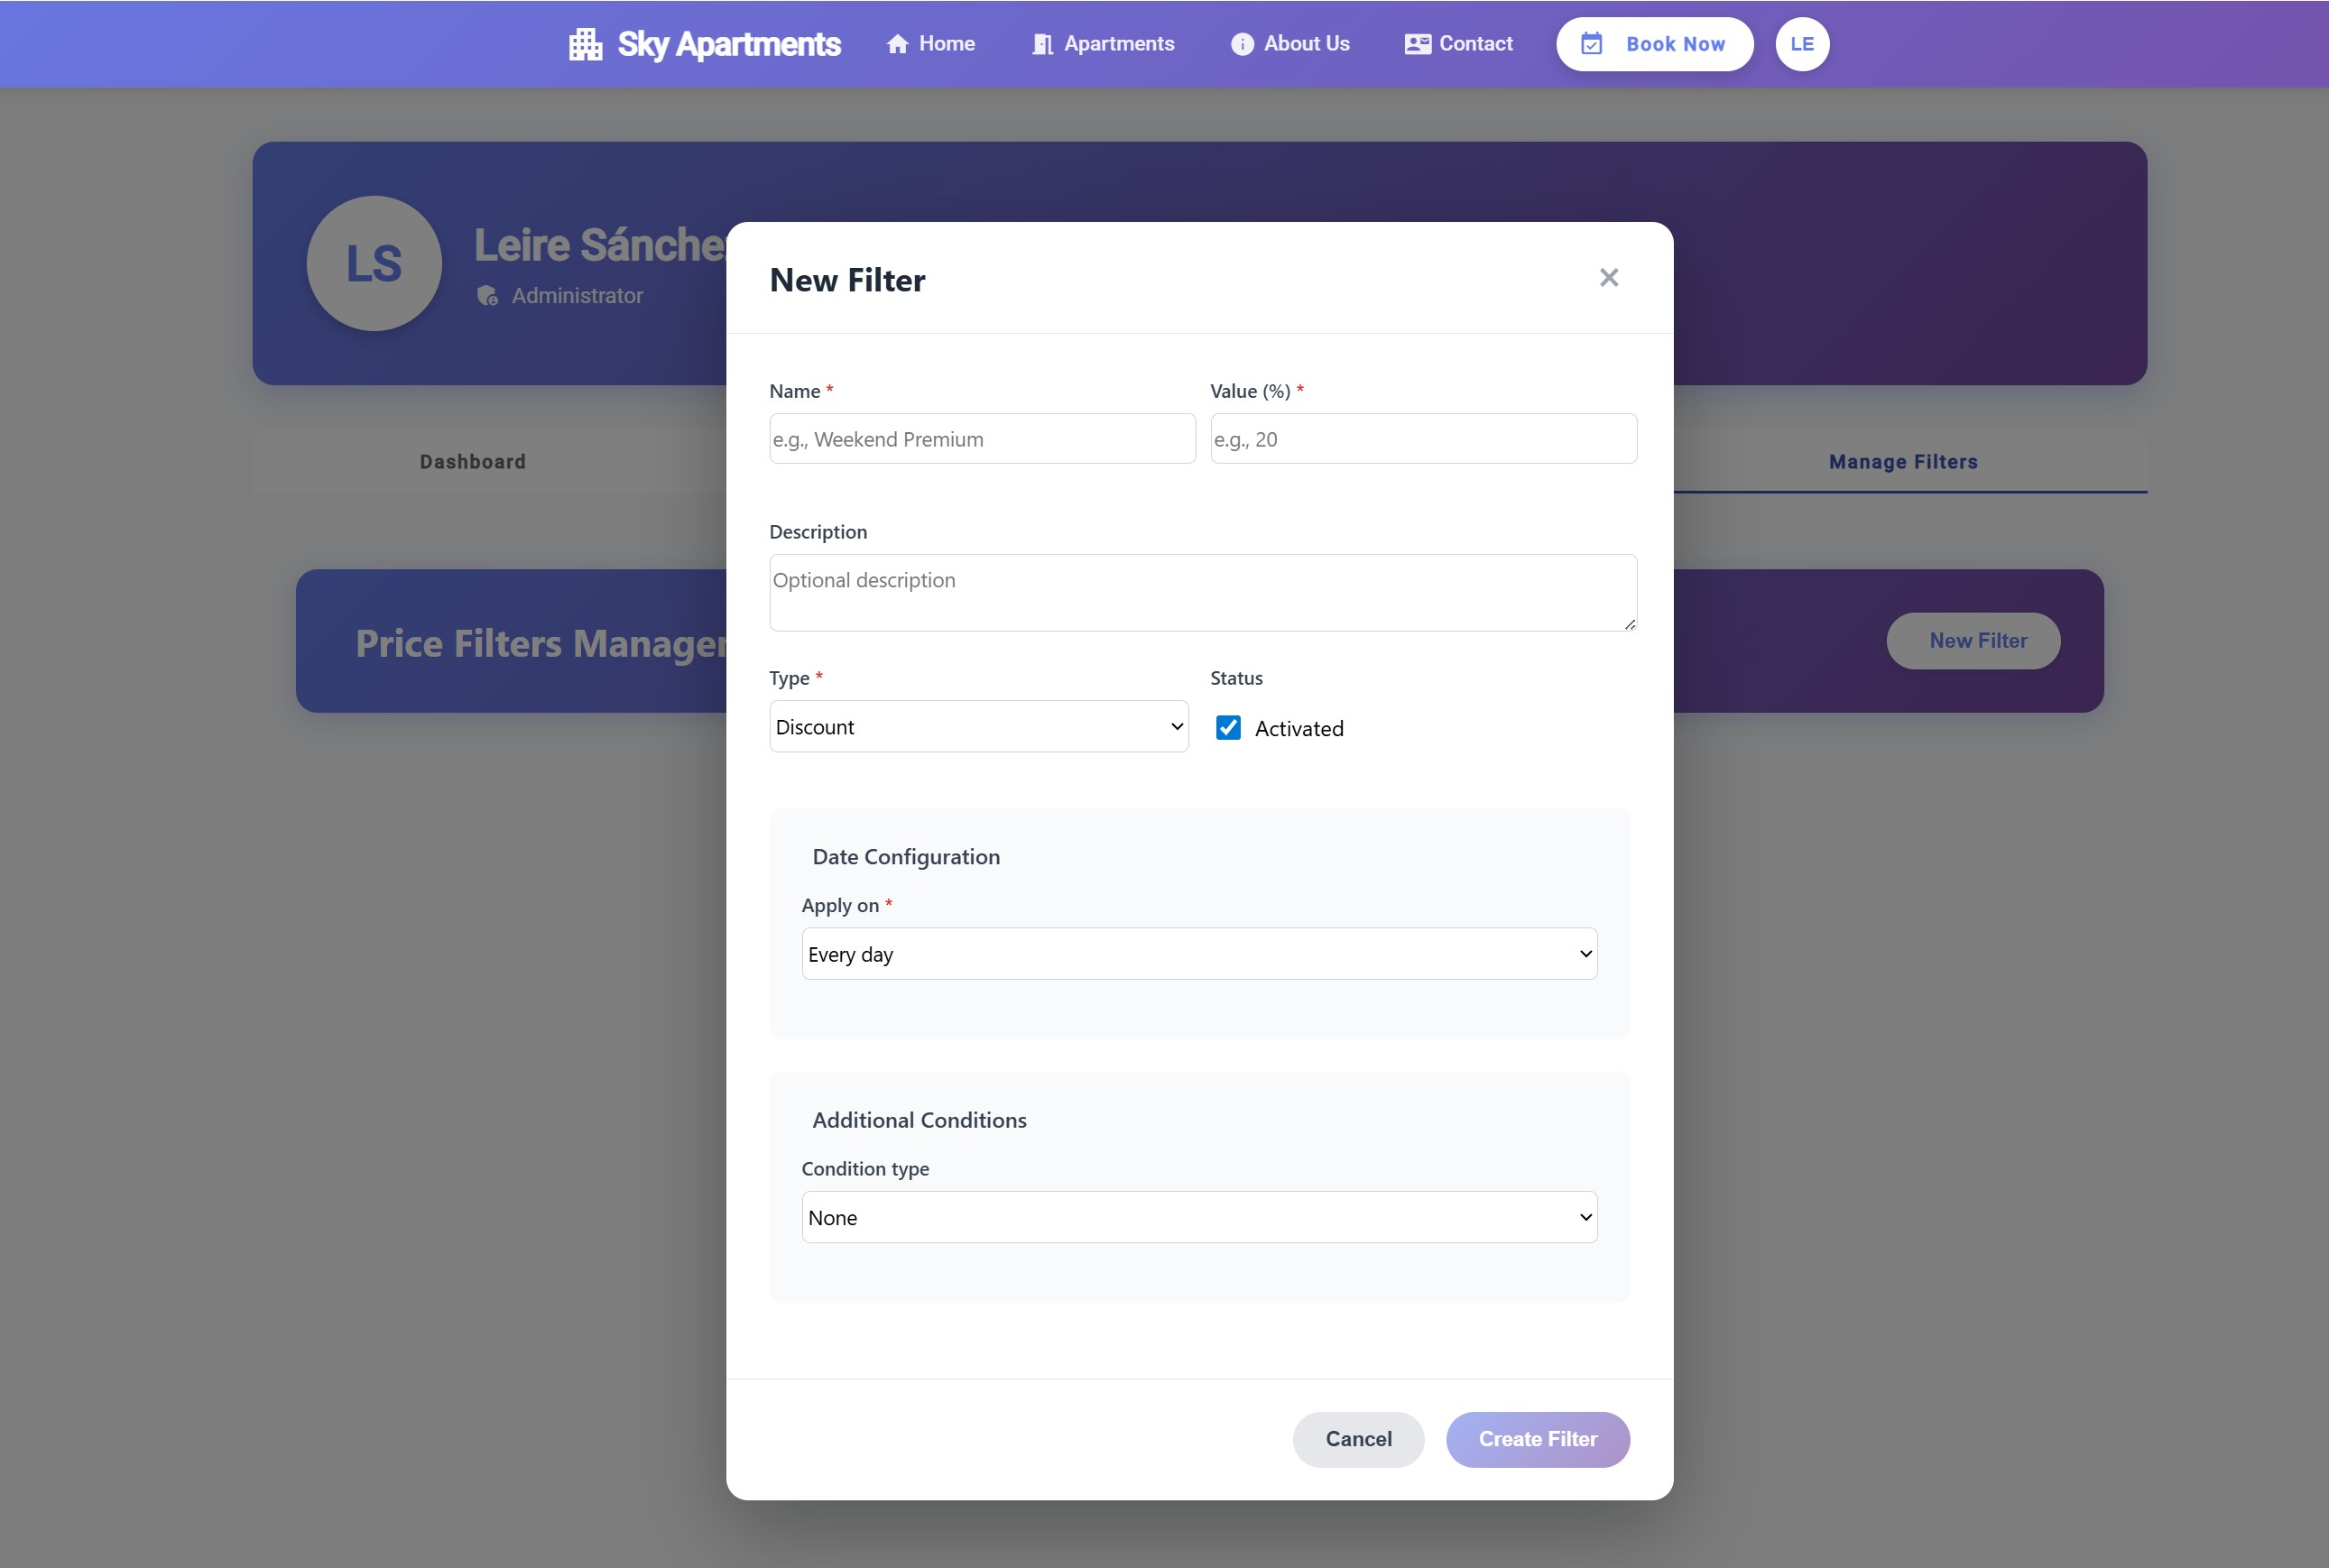
\includegraphics[width=0.8\textwidth]{img/Captura de pantalla 2026-02-23 214959.jpg}
    \caption{Modal de configuración avanzada para una nueva regla de precio dinámico.}
\end{figure}